\SourcePage{349}{354}
\section{Virtual particles}

The internal lines of Feynman diagrams play a role in invariant perturbation theory analogous to that of intermediate states in the ``ordinary'' theory. The character of these states, however, differs in the two theories. In the ordinary theory, three-dimensional momentum is conserved in intermediate states but energy is not con\SourcePageJoin{350}{355}served; in this sense they are called \emph{virtual states}. In the invariant theory, by contrast, momentum and energy enter on an equal footing: every component of 4-momentum is conserved in intermediate states. This follows because the $S$-matrix elements are integrated over both the coordinates and time, thereby making the theory invariant. What fails in an intermediate state is the relation between energy and momentum that holds for real particles, expressed by $p^2=m^2$. In this sense one speaks of intermediate \emph{virtual particles}. The relation between the momentum and energy of a virtual particle is arbitrary: it is whatever 4-momentum conservation at the vertices requires.

Consider a diagram made up of two parts, $I$ and $II$, joined by one line. Leaving their internal structure aside, represent the diagram schematically as
\begin{equation}
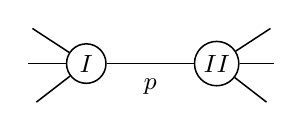
\begin{tikzpicture}[baseline=-.45ex,x=.72cm,y=.72cm,line width=.55pt,font=\small]
\node[draw,circle,inner sep=2.3pt] (I) at (-1.15,0) {$I$};
\node[draw,circle,inner sep=1.7pt] (II) at (1.15,0) {$II$};
\draw (I)--(II) node[midway,below=2pt] {$p$};
\draw (I) -- +(-.95,.62);
\draw (I) -- +(-1.02,0);
\draw (I) -- +(-.88,-.68);
\draw (II) -- +(.95,.62);
\draw (II) -- +(1.02,0);
\draw (II) -- +(.88,-.68);
\end{tikzpicture}
\tag{79.1}
\end{equation}
(the lines shown may be either solid or dashed). By overall conservation, the sums of the 4-momenta of the external lines of parts $I$ and $II$ are equal. Conservation at every vertex makes the 4-momentum $p$ of the internal line joining $I$ and $II$ equal to this same quantity. Thus this momentum is fixed uniquely and is not integrated over in the matrix element.

Depending on the reaction channel, $p^2$ may be positive or negative. There is always a channel in which $p^2>0$\footnote{For example, if energetically allowed, take the channel in which all free ends of part $I$ represent initial particles and those of part $II$ final particles. Then $p=P_i$, the sum of the 4-momenta of all initial particles, and in the center-of-momentum frame $p=(P_i^0,0)$, so $p^2>0$.}. The virtual particle then has formal properties entirely analogous to those of a real particle with a real mass $M=\sqrt{p^2}$. A rest frame can be introduced for it, its spin can be defined, and so forth.

The tensor structure of the photon propagator (76.11) is the same as the density matrix of an unpolarized massive spin-1 particle:
\[
\rho_{\mu\nu}=-\frac{1}{3}\left(g_{\mu\nu}-\frac{p_\mu p_\nu}{m^2}\right)
\]
(see (14.15)). On the other hand, the propagator, being quadratic in the field operators, plays for a virtual particle a role analogous to the density matrix of a real particle. A virtual photon must therefore be assigned spin 1, like a real photon.

\SourcePage{351}{356}
Unlike a real photon, which has two independent polarizations, a virtual photon as a finite-mass ``particle'' may have all three polarizations.

The electron propagation function has
\[
G\propto\gamma p+m.
\]
Here $m$ is the mass of a real electron, whereas the ``mass'' of the virtual particle is $M=\sqrt{p^2}$. Writing
\begin{equation}
\gamma p+m=\frac{M+m}{2M}(\gamma p+M)+\frac{M-m}{2M}(\gamma p-M),
\tag{79.2}
\end{equation}
we see that the first term corresponds to the density matrix of a mass-$M$, spin-$1/2$ particle, while the second corresponds to the density matrix of the analogous ``antiparticle'' (compare (29.10) and (29.17)). Since a particle and its antiparticle have different intrinsic parities (see \S~27), a virtual electron must be assigned the same spin $1/2$, but cannot be assigned a definite parity.

A characteristic feature of the diagram (79.1) is that it can be cut into two mutually unconnected parts by intersecting only one internal line\footnote{Almost all processes in their first nonvanishing approximation have diagrams with this property.}. In this case that line represents a \emph{one-particle} intermediate state, containing only one virtual particle. The scattering amplitude for such a diagram contains the characteristic factor, which is not integrated over,
\[
\frac{1}{p^2-m^2+i0},
\]
arising from the internal line $p$. Here $m$ is the electron mass if the line is electronic, and $m=0$ if it is photonic. Thus the scattering amplitude has a pole at those values of $p$ for which the virtual particle would become physical, $p^2=m^2$. This resembles the poles of a nonrelativistic quantum-mechanical scattering amplitude at energies corresponding to bound states of the colliding-particle system (see III, \S~128).

Consider (79.1) in the reaction channel where all right-hand free ends represent initial particles and all left-hand ends final particles, so that $p^2>0$. The initial-particle system may then be said to turn into a single virtual particle in the intermediate state. This is possible only if the transformation obeys the necessary conservation laws apart from 4-momentum conservation: conservation of angular momentum,

\SourcePage{352}{357}
charge, charge parity, and so on. This is the necessary condition for the appearance of what are called \emph{pole diagrams}. If present in one channel, crossing invariance ensures that these diagrams also occur in the other reaction channels.

For example, these conservation laws do not prevent the formation of a virtual electron through $e+\gamma\to e$. This possibility corresponds to a pole of the Compton-effect amplitude and therefore also of the amplitude in the other channel of the same reaction, two-photon annihilation of an electron pair. Formation of a virtual photon through $e^-+e^+\to\gamma$ corresponds to a pole in electron--positron scattering and hence also in electron--electron scattering. Two photons, however, can produce neither a virtual electron nor a virtual photon: $\gamma+\gamma\to e$ is forbidden by charge and angular-momentum conservation, while $\gamma+\gamma\to\gamma$ is forbidden by charge-parity conservation. Accordingly, the photon--photon scattering amplitude cannot contain pole diagrams.

The pole singularities of scattering amplitudes have here been traced from Feynman integrals, but their origin is actually more general and is not tied to perturbation theory. We shall show that they already follow from the unitarity condition (71.2).

Suppose that among the intermediate states $n$ in (71.2) there is a one-particle state. Its contribution is
\[
(T_{fi}-T_{if}^*)^{(\text{one-particle})}
=i(2\pi)^4\sum_\lambda\int\delta^{(4)}(P_f-p)T_{fn}T_{in}^*
\frac{V\,d^3p}{(2\pi)^3},
\]
where $p$ and $\lambda$ are the 4-momentum and helicity of the intermediate particle. Replace the integration over $d^3p$ by one over $d^4p$, in the region $p^0\equiv\varepsilon>0$, according to
\[
d^3p\to2\varepsilon\delta(p^2-M^2)d^4p
\]
where $M$ is the mass of the intermediate particle. The integration removes the delta function $\delta^{(4)}(P_f-p)$. Then changing from $T_{fi}$ to $M_{fi}$ according to (64.10), we find
\begin{equation}
(M_{fi}-M_{if}^*)^{(\text{one-particle})}
=2\pi i\delta(p^2-M^2)\sum_\lambda M_{fn}M_{in}^*.
\tag{79.3}
\end{equation}

Assuming $T$ and $P$ invariance, we have, up to a phase factor, $M_{if}=M_{f'i'}$, where $i'$ and $f'$ differ from $i$ and $f$ only in the signs of the particle helicities, at unchanged momenta. Adding (79.3) to the analogous equation for $M_{f'i'}-M_{i'f'}^*$ gives
\begin{equation}
\operatorname{Im}\overline M_{fi}^{(\text{one-particle})}
=-\pi\delta(p^2-M^2)R,
\tag{79.4}
\end{equation}

\SourcePage{353}{358}
where
\[
\overline M_{fi}=M_{fi}+M_{f'i'},
\qquad
R=-\sum_\lambda\bigl(M_{fn}M_{in}^*+M_{f'n}M_{i'n}^*\bigr).
\]
It follows that $\overline M_{fi}$, as an analytic function of $p^2=P_i^2=P_f^2$, has a pole at $p^2=M^2$. According to (75.18), its pole part is
\begin{equation}
\overline M_{fi}^{(\text{one-particle})}
=\frac{R}{p^2-M^2+i0}.
\tag{79.5}
\end{equation}
Real transitions to a one-particle state are possible only when $P_i^2=P_f^2$ equals $M^2$. Thus we have indeed obtained the scattering-amplitude structure corresponding to a diagram of the form (79.1).

Finally, consider an important property of diagrams containing closed electron loops. It follows readily by applying the notion of charge parity to a virtual photon: a virtual photon, like a real one, must be assigned a definite negative charge parity\footnote{This follows from the same considerations concerning the electromagnetic-interaction operator acting at each vertex that were given in \S~13 for a real photon.}.

If a diagram contains a closed loop with $N>2$ vertices, the amplitude for the process must also include another diagram differing only in the direction in which the loop is traversed. For $N=2$, a direction of traversal plainly has no meaning. ``Cut out'' the loops along the dashed lines leading to them. This gives two loops, $\Pi_{\mathrm I}$ and $\Pi_{\mathrm{II}}$:
\begin{equation}
\begin{gathered}
\begin{tikzpicture}[baseline=-.45ex,x=.58cm,y=.58cm,>=Stealth,line width=.55pt,font=\small]
\foreach \a in {90,18,-54,-126,162} {
  \draw[dashed] ({1.02*cos(\a)},{1.02*sin(\a)}) -- ({1.55*cos(\a)},{1.55*sin(\a)});
}
\coordinate (a) at (90:1.02); \coordinate (b) at (18:1.02);
\coordinate (c) at (-54:1.02); \coordinate (d) at (-126:1.02);
\coordinate (e) at (162:1.02);
\draw[->] (a)--(b); \draw[->] (b)--(c); \draw[->] (c)--(d);
\draw[->] (d)--(e); \draw[->] (e)--(a);
\node at (0,0) {$\Pi_{\mathrm I}$};
\end{tikzpicture}
\qquad\qquad
\begin{tikzpicture}[baseline=-.45ex,x=.58cm,y=.58cm,>=Stealth,line width=.55pt,font=\small]
\foreach \a in {90,18,-54,-126,162} {
  \draw[dashed] ({1.02*cos(\a)},{1.02*sin(\a)}) -- ({1.55*cos(\a)},{1.55*sin(\a)});
}
\coordinate (a) at (90:1.02); \coordinate (b) at (18:1.02);
\coordinate (c) at (-54:1.02); \coordinate (d) at (-126:1.02);
\coordinate (e) at (162:1.02);
\draw[<-] (a)--(b); \draw[<-] (b)--(c); \draw[<-] (c)--(d);
\draw[<-] (d)--(e); \draw[<-] (e)--(a);
\node at (0,0) {$\Pi_{\mathrm{II}}$};
\end{tikzpicture}
\end{gathered}
\tag{79.6}
\end{equation}
They may be regarded as diagrams defining the amplitude for transforming one collection of photons, real or virtual, into another; $N$ is then the sum of the numbers of initial and final photons. Charge-parity conservation forbids an even number of photons from turning into an odd number. Therefore, for odd $N$, the sum of the expressions corresponding to the loops (79.6) must vanish. Hence the combined contribution to the scattering amplitude of the two diagrams containing these loops as compo\SourcePageJoin{354}{359}nents also vanishes. This is \emph{Furry's theorem} (W.~H.~Furry, 1937).

Thus, in constructing the amplitude of any process, diagrams containing loops with an odd number of vertices need not be considered at all.

Let us trace the origin of this mutual cancellation more closely. For specified photon-line momenta $k_1,k_2,\ldots,k_N$, a closed electron loop corresponds to the expression
\begin{equation}
\int d^4p\cdot\Tr\bigl[(\gamma e_1)G(p)(\gamma e_2)G(p+k_1)\ldots\bigr],
\tag{79.7}
\end{equation}
where $p,p+k_1,\ldots$ are the electron-line momenta, which remain incompletely determined after the conservation laws at the vertices have been applied. Perform charge conjugation on all matrices $\gamma^\mu$ and $G$, replacing them by $U_C^{-1}\gamma^\mu U_C$ and $U_C^{-1}GU_C$. This leaves (79.7) unchanged because the trace of a matrix product is invariant under such a transformation. On the other hand, by (26.3),
\begin{equation}
U_C^{-1}\gamma^\mu U_C=-\widetilde\gamma^\mu,
\tag{79.8}
\end{equation}
and therefore
\begin{equation}
U_C^{-1}G(p)U_C
=\frac{-p\widetilde\gamma+m}{p^2-m^2}
=\widetilde G(-p).
\tag{79.9}
\end{equation}
Replacing $G(p)$ by the transposed matrix with the sign of $p$ reversed plainly changes the direction in which the loop is traversed, reversing every arrow. Thus the transformation takes one loop into the other and produces a factor $(-1)^N$ from the substitution (79.8) at every vertex. Hence
\begin{equation}
\Pi_{\mathrm I}=(-1)^N\Pi_{\mathrm{II}},
\tag{79.10}
\end{equation}
so the two loop contributions are equal for even $N$ and opposite in sign for odd $N$.
